\FloatBarrier
\begin{figure}
	\begin{subfigure}[t]{0.5\textwidth}
		\centering
		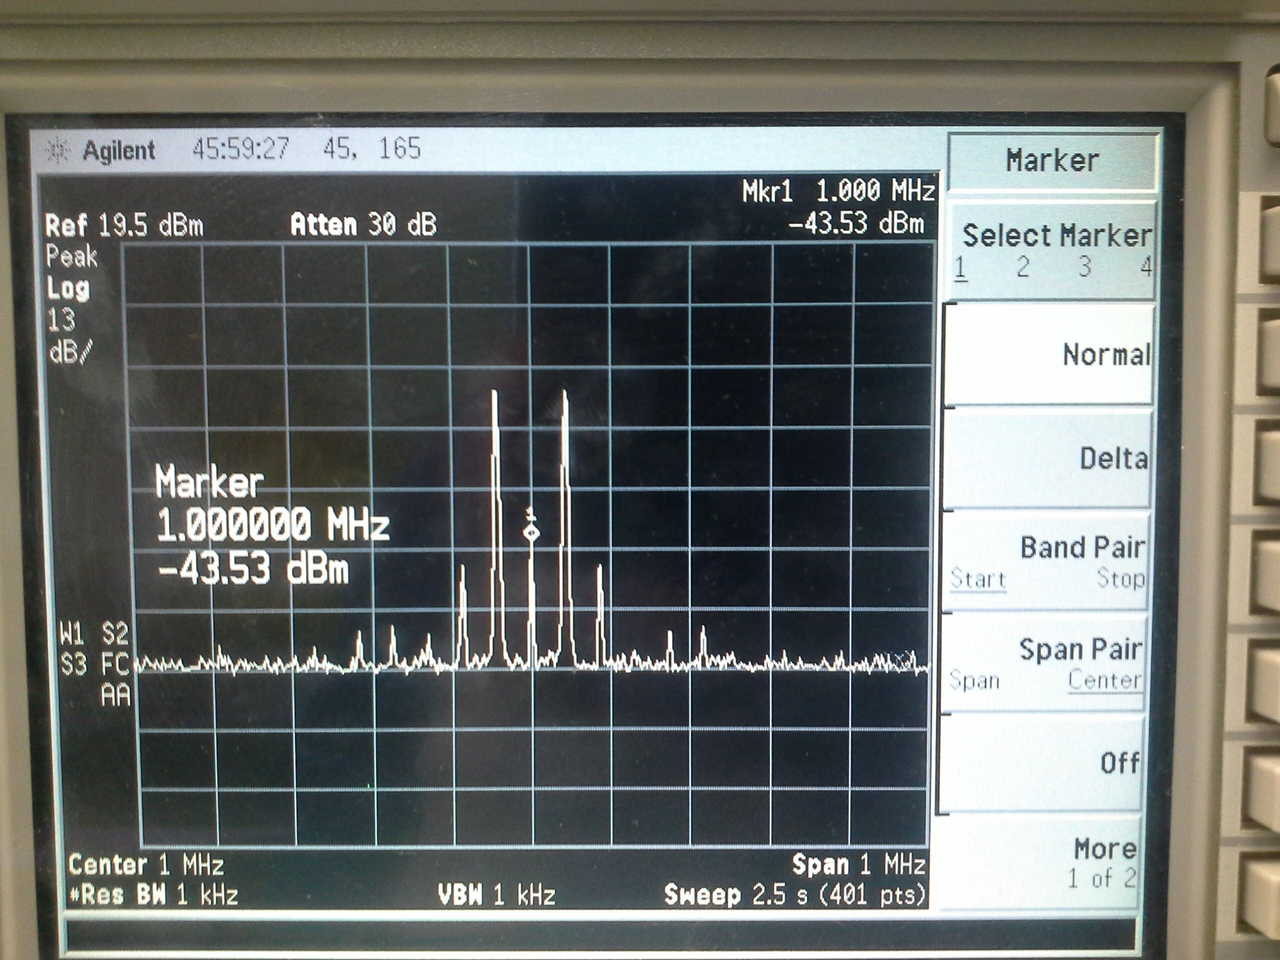
\includegraphics[scale=0.17]{../Grafiken/Frequenzspektrum_b_AmpModuliertTraegerunterdrueckung_0.jpg}
		\caption{Trägerfrequenz\label{fig:frequenzspektrum_b_ampmodulierttraegerunterdrueckung_0}}
	\end{subfigure}%
	~
	\begin{subfigure}[t]{0.5\textwidth}
		\centering
		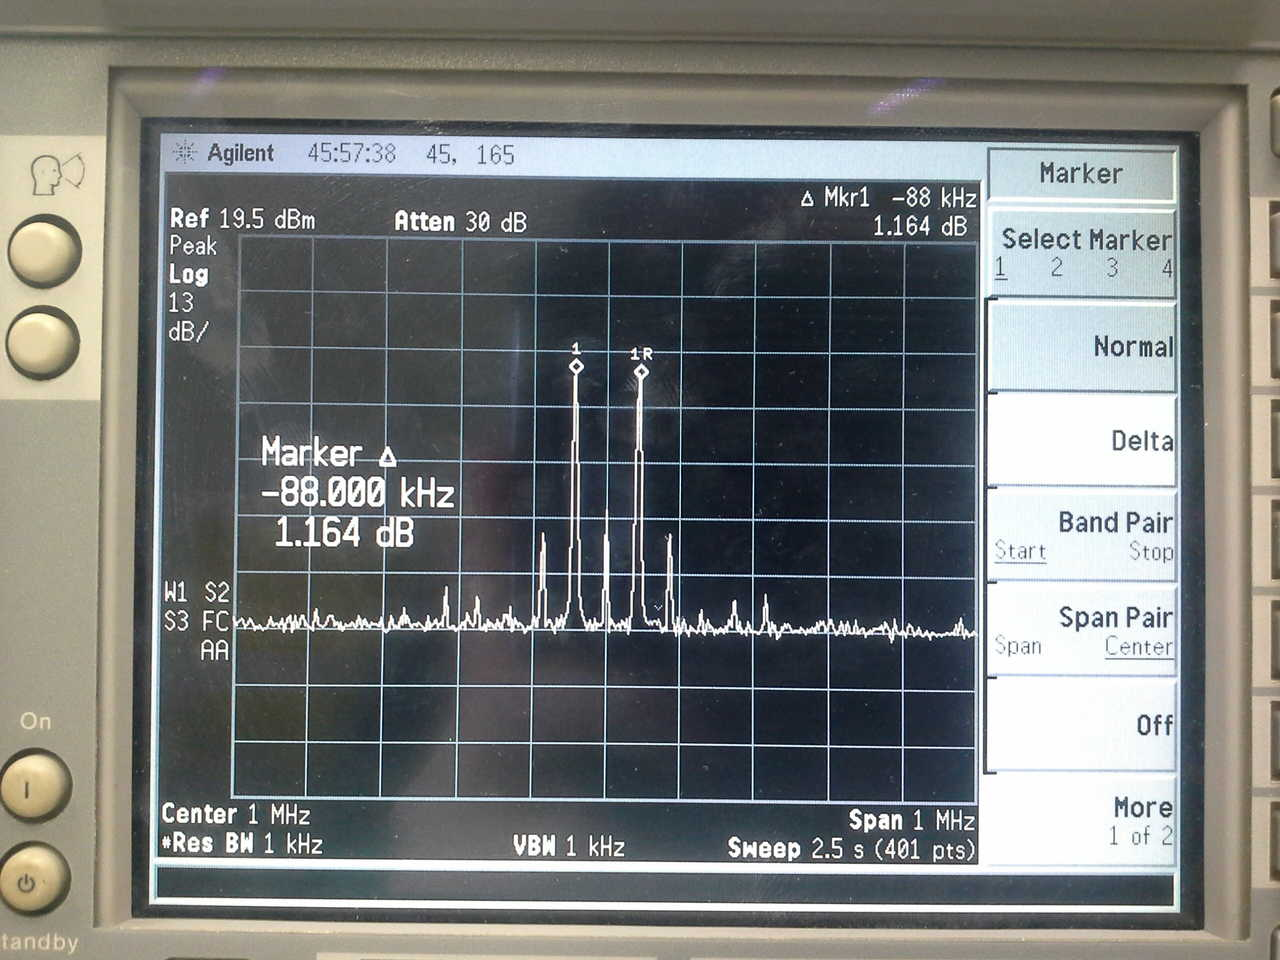
\includegraphics[scale=0.17]{../Grafiken/Frequenzspektrum_b_AmpModuliertTraegerunterdrueckung_1.jpg}
		\caption{Frequenzunterschied der Seitenbänder \label{fig:frequenzspektrum_b_ampmodulierttraegerunterdrueckung_1}}
	\end{subfigure}
	\caption{Frequenzspektrum der amplitudenmodulierten Spannung mit Trägerunterdrückung. Dargestellt ist 
		die Trägerfrequenz (a) und der Frequenzunterschied der ersten beiden Seitenbänder (b).
		\label{fig:frequenzspektrum_b_ampmodulierttraegerunterdrueckung}}
\end{figure}
\FloatBarrier